\section{Exploits}
In dieser Aufgabe sollten Sie folgende Angriffe durchführen. Dokumentieren und erklären Sie die
einzelnen Angriffe kurz und knapp. Dokumentieren Sie auch, dass und wie Sie alle hier genutzten
Schwachstellen in Aufgabe 1 gefunden haben.

\subsection{Begrifflichkeiten}
\textit{Erklären Sie den Unterschied zwischen Bind\_shell, Reverse\_shell sowie staged und non-staged Payloads.}

\subsubsection{Vergleich: Bind\_shell vs. Reverse\_shell}
\begin{center}
    \begin{tabular}{|p{4cm}|p{4cm}|}
        \hline
        \textbf{Bind\_shell (Direct Payload)} & \textbf{Reverse\_shell (Reverse Payload)} \\ 
        \hline
        Der Angreifer verbindet sich mit dem Opfer. & Das Opfer verbindet sich mit dem Angreifer. \\ \hline
    \end{tabular}
\end{center}


\subsubsection{Vergleich: staged vs. non-staged Payload}
\begin{center}
    \begin{tabular}{|p{6cm}|p{6cm}|}
        \hline
        \textbf{staged Payload} & \textbf{non-staged Payload} \\
        \hline
        Staged Payloads unterteilen den Delivery-Prozess in zwei Schritte. Initial wird ein sogenannter Stager an das Zielsystem delivered. Dieser etabliert die Kommunikation und lädt anschließend den korrekten Payload herunter. Dadurch wird die initiale Payload-Size verringert, der Angreifer kann den zweiten Payload anpassen und der Payload umgeht gegebenenfalls Intrusion Detection System (IDS). & 
        Non-Staged Payloads liefern den vollständigen Payload auf einmal. Dadurch entfallen die Vorteile der Staged-Variante. Die Vorteile dieser Variante sind jedoch Simplicity, Speed und Predictable Behavior. \\
        \hline
    \end{tabular}
\end{center}

% ======================================================================================================
\subsection{Angriff mittels Reverse Shell und John the Ripper}
\textit{Greifen Sie Windows XP mittels dem Exploit ms08\_067\_netapi an und eröffnen Sie eine Meterpretersession mittels einer reverse\_shell. Erweitern Sie ihre Rechte und laden Sie die gespeicherten Windows Lan-Manager Hashes herunter. Ermitteln Sie die dazugehörigen Passwörter mittels eines geeigneten Passwortcrackers z.B. John the Ripper. Funktioniert der Angriff auch mit einer bind\_shell. Geben Sie eine Erklärung dafür. Warum macht es Sinn sich Login-Daten zu verschaffen, auch wenn man bereits durch einen exploit Zugriff auf das System hat? Erklären Sie in einem Satz, welche Schwäche obiger Exploit ausnutzt.}\\

Für diesen Angriff wird der Exploit
\begin{center}
    \texttt{windows/smb/ms08\_067\_netapi}
\end{center}
verwendet. Als Konfigurationsdaten werden das Opfer als \texttt{RHOST} und der Angreifer als \texttt{LHOST} gesetzt. Außerdem wird die zu verwendende \texttt{PAYLOAD}
\begin{center}
    windows/meterpreter/reverse\_tcp
\end{center}
gesetzt. \autoref{fig:peter_success} zeigt diese Einstellungen und die erfolgreiche Ausführung des Exploits.
%\begin{figure}[H]
%    \centering
%    
\includegraphics[width=0.85\linewidth]{Whakaahua/aufgabe2/b/peter_config.png}
%    \caption{ms08\_067\_netapi: Konfigurationen}
%    \label{fig:peter_config}
%\end{figure} \noindent
\begin{figure}[H]
    \centering
    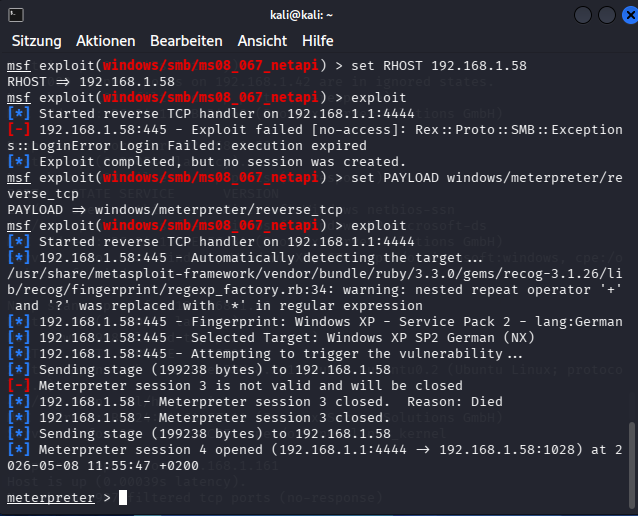
\includegraphics[width=0.85\linewidth]{Whakaahua/aufgabe2/b/peter_success.png}
    \caption{ms08\_067\_netapi + reverse\_tcp}
    \label{fig:peter_success}
\end{figure} \noindent
Nach erfolgreichem Login wird \texttt{\$ hashdump} ausgeführt, was uns die Hashes liefert, zu sehen in \autoref{fig:peter_hashdump}.
\begin{figure}[H]
    \centering
    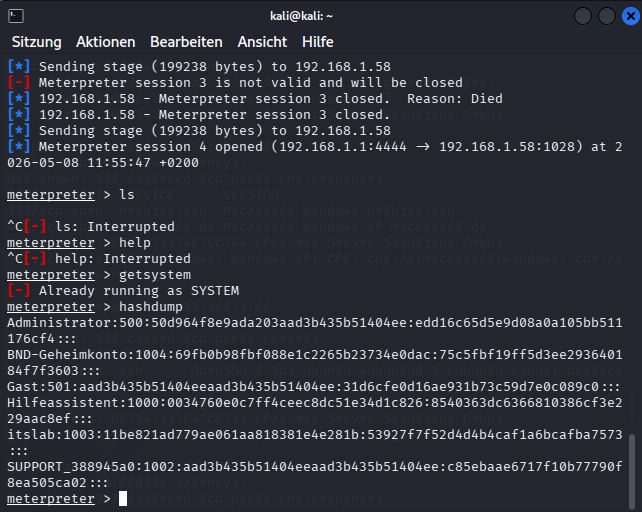
\includegraphics[width=0.85\linewidth]{Whakaahua/aufgabe2/b/peter_hashdump.png}
    \caption{Meterpreter: Hashdump}
    \label{fig:peter_hashdump}
\end{figure} \noindent
Mittels \texttt{John the Ripper} können diese geknackt werden. Dieses CLI-Tool nimmt eine hashlist entgegen und Argumente, wie diese geknackt werden soll. \autoref{fig:john_wordlist} zeigt die Wordlist-Option, bei dem ein Dictionary-Angriff auf die Passwörter durchgeführt wird. Es werden ein paar Erfolge verzeichnet, allerdings nicht vollständig.
\begin{figure}[H]
    \centering
    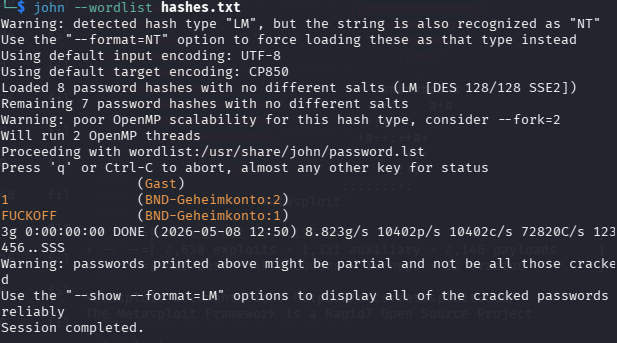
\includegraphics[width=0.85\linewidth]{Whakaahua/aufgabe2/b/john_wordlist.png}
    \caption{John the Ripper: Wordlist}
    \label{fig:john_wordlist}
\end{figure} \noindent
\autoref{fig:john_4von5} zeigt, dass ein Paar Passwörter gefunden worden sind, aber nicht alle.
\begin{figure}[H]
    \centering
    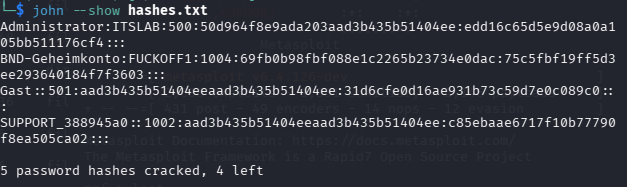
\includegraphics[width=0.85\linewidth]{Whakaahua/aufgabe2/b/john_4von5.png}
    \caption{John the Ripper: Fast fertig}
    \label{fig:john_4von5}
\end{figure} \noindent
\autoref{fig:john_incremental} zeigt die Verwendung der Incremental-Funktion, die einen Bruteforce durchführt.
\begin{figure}[H]
    \centering
    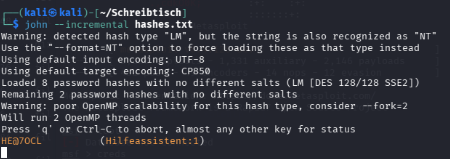
\includegraphics[width=0.85\linewidth]{Whakaahua/aufgabe2/b/john_incremental.png}
    \caption{John the Ripper: Incremental}
    \label{fig:john_incremental}
\end{figure} \noindent
Mit etwas Geduld wird der Angriff erfolgreich, zu sehen in \autoref{fig:john_fertig}.
\begin{figure}[H]
    \centering
    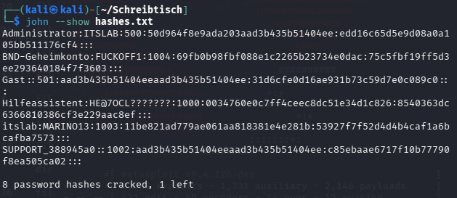
\includegraphics[width=0.85\linewidth]{Whakaahua/aufgabe2/b/john_fertig.png}
    \caption{John the Ripper: Erfolg}
    \label{fig:john_fertig}
\end{figure} \noindent

% ======================================================================================================
\subsection{Angriff auf einen Gitlab-Server (vorübergehender Titel)}

\textit{Greifen Sie den Gitlab Server an. Der Exploit muss hier selbst bestimmt werden. Die hier verwendete Gitlab Version ist dabei 12.4.0. Die IP des Servers ist zuvor durch Aufgabe 1. ermittelt worden.}

\textit{Ein anfälliger Account ist dabei victim mit dem Passwort 12345678. Dieser Angriff funktioniert aber auch ohne vorher bekannten Nutzer, Sie müssten sich nur selbst am Server registrieren (was hier wegen dem fehlenden Mailserver und Internet nicht so ohne weiteres geht.). Ermitteln Sie den Inhalt der Datei flag.loot auf dem Server.}

Wir haben den Gitlab Server identifiziert in unserem NMAP Scan aus Aufgabe 1 und festegestellt es ist die 192.168.1.66.
\\
Haben dann folgend dadurch, dass uns die Version bekannt ist geschaut was Metasploit für Exploits anbietet für diese Version und sind über das Modul gitlab-file-read-rce gestoßen, mitdem wir es hinbekommen eine Reverse-Shell zu injezieren.
\begin{figure}[H]
	\centering
	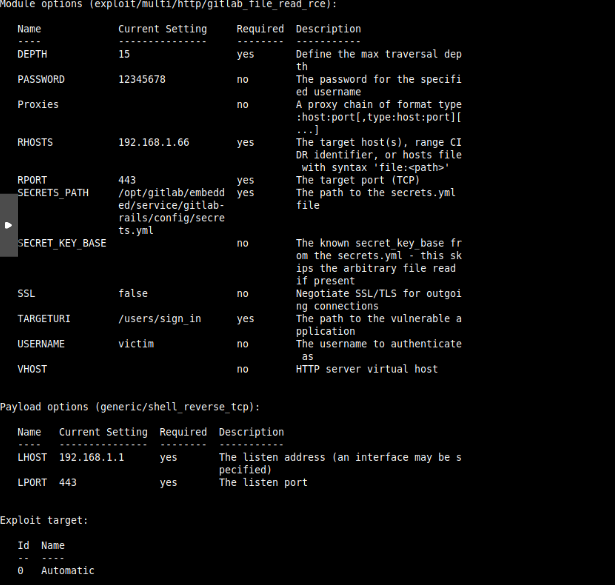
\includegraphics[width=0.85\linewidth]{Whakaahua/aufgabe2/Gitlab_angriff_optionen.png}
	\caption{Optionen für Gitlab\_angriff}
	\label{fig:GitlabOptionen}
\end{figure} \noindent
Nach Ausführung des Exploits haben wir eine Verbindung zu dem Gitlab-Server:
\begin{figure}[H]
	\centering
	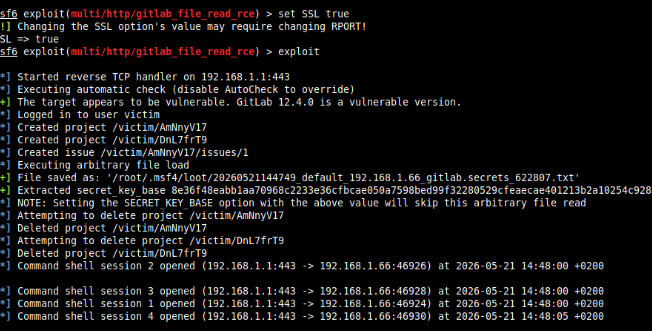
\includegraphics[width=0.85\linewidth]{Whakaahua/aufgabe2/Gitlab_exploit_start.png}
	\caption{Exploit und Sessions open}
\label{fig:SessionOpen}
\end{figure}
Nun mussten wir aber Feststellen, dass die Shells die Benutzt wurden nicht ausreichend sind und zu wenig Rechte haben um das Flag auszulesen. Daher haben wir die Session und Verbindung die nicht Ruby ist Upgraded auf eine Meterpreter Shell.
\begin{figure}[H]
	\centering
	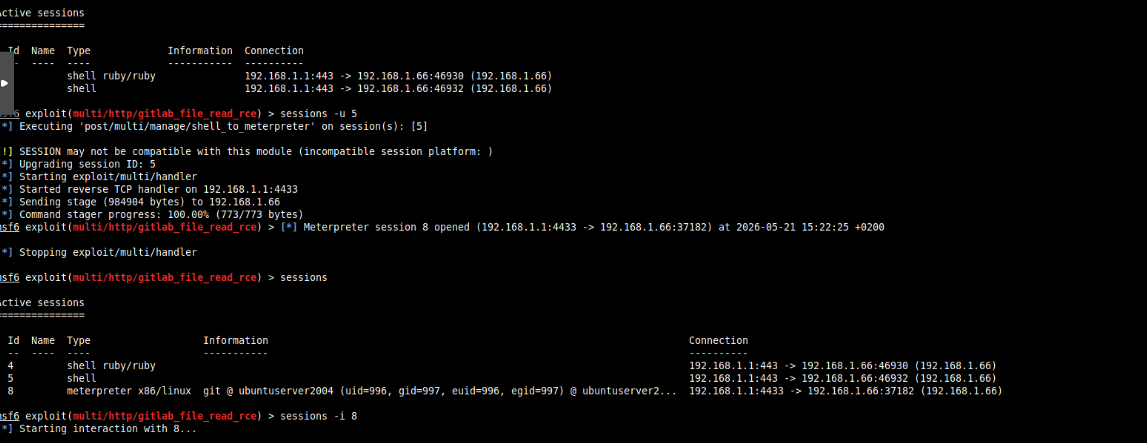
\includegraphics[width=0.85\linewidth]{Whakaahua/aufgabe2/Gitlab_habenmeterpreter.png}
	\caption{Upgrade auf Meterpreter Session}
\label{fig:Meterpreter}
\end{figure}
Schlussendlich mit der Meterpreter-Shell hatten wir dann genügend Rechte um das gesuchte Flag auslesen zu können\\
\begin{figure}[H]
	\centering
	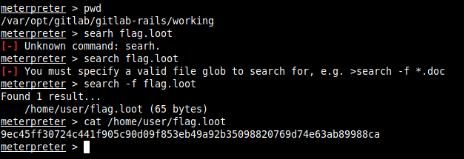
\includegraphics[width=0.85\linewidth]{Whakaahua/aufgabe2/Gitlab_haben_flag.png}
	\caption{Flag}
\label{fig:GitlabFlag}
\end{figure}


\subsection{Angriff auf mssql}
\textit{Greifen Sie den weiteren XP-Rechner mittels \texttt{mssql\_login} an und verschaffen sich Sie Zugriff zum System mittels \texttt{mssql\_payload}.}\\

\noindent Der Angriff wird via Metasploit durchgeführt. Der Angriff ist unter dem Path
\begin{center}
    \texttt{scanner/mssql/mssql\_login}
\end{center}
zu finden. Der Pfad konnte über einen einfachen \texttt{find}-Befehl ermittelt werden. Per \texttt{use}-Befehl in der msfconsole wird der Angriff ausgewählt. Dieser benötigt die Parameter \texttt{RHOST} := 192.168.1.32 und \texttt{RPORT} := 1113. Letzterer war deshalb besonders relevant, da der Standardport für diesen Angriff geschlossen ist. Außerdem erhält der Angriff die Wörterliste
\begin{center}
    \texttt{/usr/share/wordlists/rockyou.txt}
\end{center}
(Parameter \texttt{PASS\_FILE}), welche aber zunächst entpackt werden muss. Weitere wichtige Konfigurationen sind in \autoref{fig:mssql_login_show_options} zu sehen.
\begin{figure}[H]
    \centering
    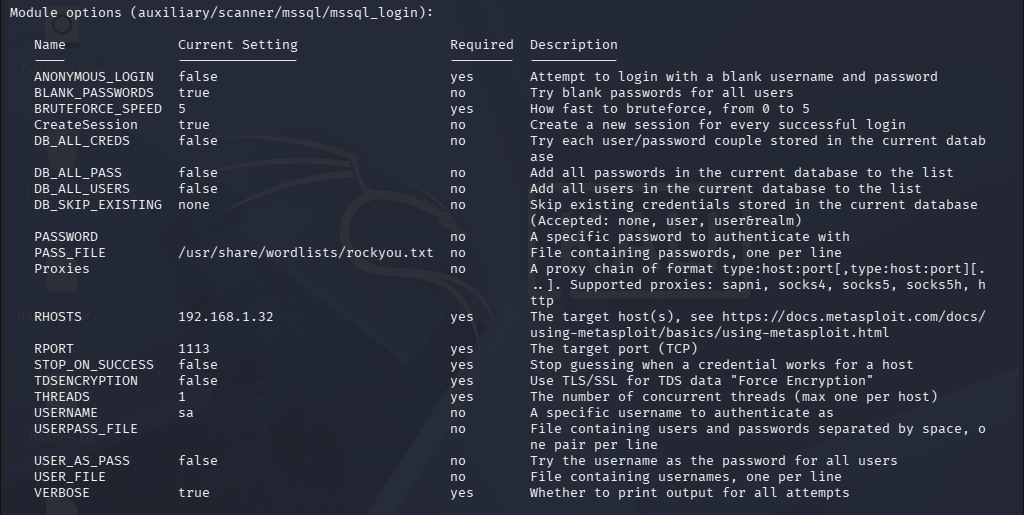
\includegraphics[width=0.85\linewidth]{Whakaahua/aufgabe2/d/mssql_login_show_options.png}
    \caption{Options for \texttt{mssql\_login}}
    \label{fig:mssql_login_show_options}
\end{figure} \noindent
Mit den korrekten Konfigurationen wird der Exploit gestartet. Alle Passwörter der Wörterliste werden durchprobiert. Das Ergebnis des erfolgreichen Durchlaufs ist in \autoref{fig:mssql_login_exploit} zu sehen.
\begin{figure}[H]
    \centering
    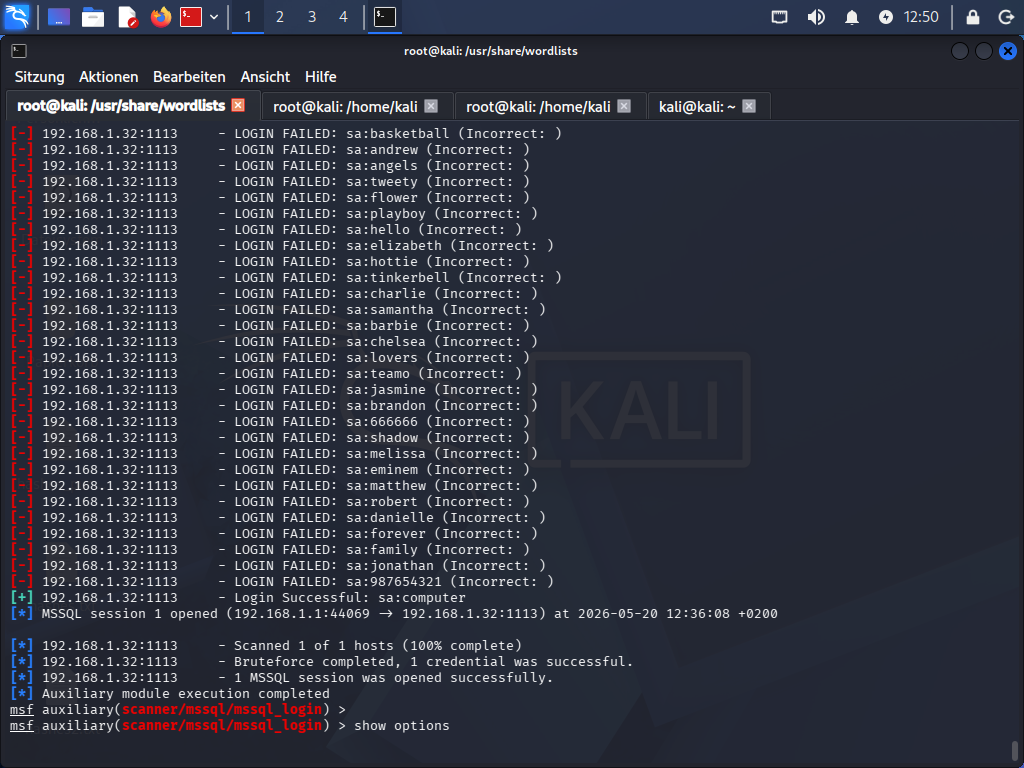
\includegraphics[width=0.85\linewidth]{Whakaahua/aufgabe2/d/mssql_login_exploit.png}
    \caption{\texttt{mssql\_login}}
    \label{fig:mssql_login_exploit}
\end{figure} \noindent
Mit den gefundenen Anmeldedaten \texttt{sa:computer} für den Admin kann nun der Exploit \texttt{mssql\_payload} verwendet werden.
Dieser ist unter dem Pfad
\begin{center}
    \texttt{windows/mssql/mssql\_payload}
\end{center}
zu finden. \autoref{fig:mssql_payload_show_options} zeigt die wichtigsten Konfigurationen für den Exploit, darunter wieder \texttt{RHOST} := 192.168.1.32 und \texttt{RPORT} := 1113, aber diesmal auch \texttt{USERNAME} := sa und \texttt{PASSWORD} := computer.
\begin{figure}[H]
    \centering
    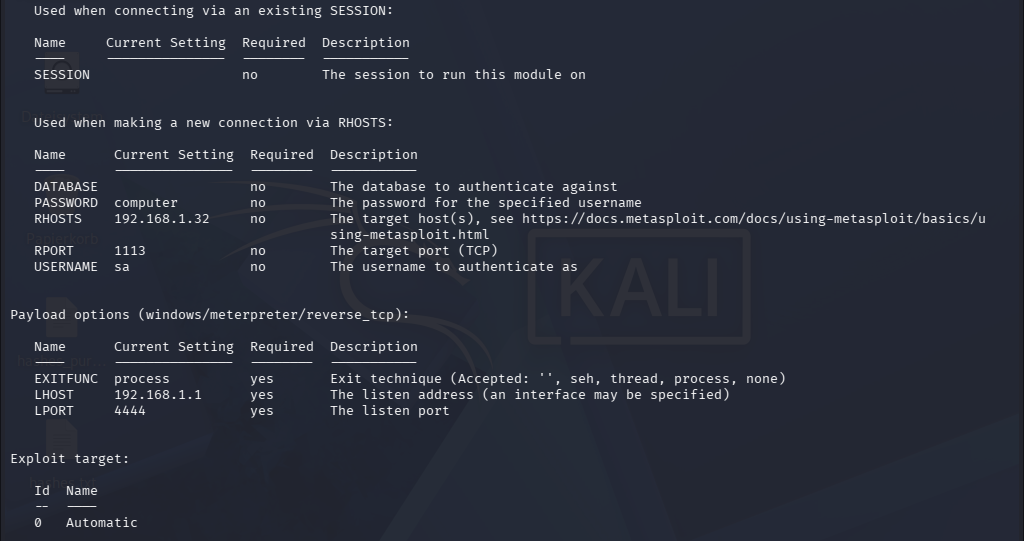
\includegraphics[width=0.85\linewidth]{Whakaahua/aufgabe2/d/mssql_payload_show_options.png}
    \caption{Options for \texttt{mssql\_payload}}
    \label{fig:mssql_payload_show_options}
\end{figure} \noindent
Der Befehl \texttt{exploit} startet den Angriff. Der Vorgang und das Ergebnis sind in \autoref{fig:mssql_payload_exploit} zu sehen.
\begin{figure}[H]
    \centering
    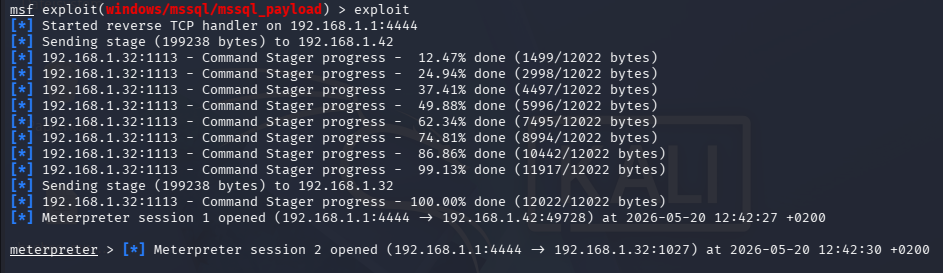
\includegraphics[width=0.85\linewidth]{Whakaahua/aufgabe2/d/mssql_payload_exploit.png}
    \caption{\texttt{mssql\_payload}}
    \label{fig:mssql_payload_exploit}
\end{figure} \noindent
Das Ergebnis ist eine Meterpreter-Shell (reverse\_shell). Der Angriff war ein Erfolg.